%------------------------------------------------------------------------------
% SMURF Paper
%------------------------------------------------------------------------------

\documentclass[useAMS,usenatbib,nofootinbib]{mn2e}

% this is needed to get pdftex to work properly!
\usepackage[pdftex]{graphicx}

\usepackage{amsmath}
\usepackage{url}
\usepackage{natbib}
\usepackage{rotating}

% --- Some user defined macros ------------------------------------------------

% journals
\newcommand{\apj}{\rm ApJ}
\newcommand{\apjl}{\rm ApJL}
\newcommand{\apjs}{\rm ApJS}
\newcommand{\aaps}{\rm A$\&$AS}
\newcommand{\aap}{\rm A$\&$A}
\newcommand{\aapr}{\rm A$\&$AR}
\newcommand{\mnras}{\rm MNRAS}
\newcommand{\aj}{\rm Astron. J.}
\newcommand{\araa}{\rm ARAA}
\newcommand{\nat}{\rm Nature}
\newcommand{\pasj}{\rm PASJ}
\newcommand{\pasp}{\rm Publ. Astron. Soc. Pac.}
\newcommand{\prd}{\rm PhRvD}
\newcommand{\ASP}{\rm ASP Conference Series}
\newcommand{\CASP}{\rm Comm. Astrophys. Space Phys.}
\newcommand{\astroph}{\rm astro-ph/}


% common acronyms etc.
\newcommand{\snr}{SNR}
\newcommand{\scuba}{SCUBA-2}
\newcommand{\rms}{RMS}

% these are approximately less-than and greater-than symbols
\def\lsim{\mathrel{\lower2.5pt\vbox{\lineskip=0pt\baselineskip=0pt
          \hbox{$<$}\hbox{$\sim$}}}}

\def\gsim{\mathrel{\lower2.5pt\vbox{\lineskip=0pt\baselineskip=0pt
          \hbox{$>$}\hbox{$\sim$}}}}


% ----------------------------------------------------------------------------

\title[SMURF: an iterative map-maker for SCUBA-2]{The Sub-Millimetre User
Reduction Facility: an iterative map-maker for SCUBA-2}

\author[Edward~L.~Chapin~et~al.]{
  \parbox[t]{\textwidth}{
    Edward~L.~Chapin$^{1}$\thanks{E-mail:~echapin@phas.ubc.ca},
    David~S.~Berry$^{2}$,
    Andrew~G.~Gibb$^{1}$,
    Tim~Jenness$^{2}$,
    Douglas~Scott$^{1}$
  }
  \\
  \\
  $^{1}$Dept. of Physics \& Astronomy, University of British Columbia,
  6224 Agricultural Road, Vancouver, B.C. V6T 1Z1, Canada\\
  $^{2}$JointAstronomy Centre, 660 N. A`oh\={o}k\={u} Place, University
  Park, Hilo, Hawaii 96720, USA}

\begin{document}

\label{firstpage}

\maketitle

\begin{abstract}
  We describe the properties of data from the Submillimetre Common
  User Bolometer Array 2 (SCUBA-2) taken during the Shared Risk
  Observing period from 2010 February 11 to 2010 March 25, and the
  production of maps using the Sub-Millimetre User Reduction Facility
  (SMURF). Our iterative approach is similar to those used to reduce
  data from other ground-based submillimetre telescopes in recent
  years, and recovers angular scales up to the size of the array
  footprint (approximately 2\,arcmin). The method is also able to
  achieve the theoretical white-noise limit of the instrument for
  point-source studies.
\end{abstract}


\begin{keywords}
chicken, chicken: chicken, chicken: chicken -- chicken
\end{keywords}

%------------------------------------------------------------------------------
\section{Introduction}
\label{sec:intro}
%------------------------------------------------------------------------------

\textbf{Guideline for figures:}

\begin{itemize}
\item minimize excess whitespace around the figure to optimize usage of space
\item ensure a decent line thickness
\item use a Times font for labels with a thickness that resembles the
  text in the body. The font size should be similar to the main body
  text or larger
\item avoid using colour unless it is necessary for emphasis
\end{itemize}

\textbf{start intro here...}

The Submillimetre Common User Bolometer Array 2
\citep[\scuba,][]{holland2006} is a new instrument for the 15-m
James Clerk Maxwell Telescope (JCMT) on Mauna Kea, Hawai'i. The camera
can simultaneously image the sky in two broad bands centered over 450
and 850\,\micron. Ultimately, the instrument will also be equipped
with a Fourier transform spectrometer \citep[FTS-2,][]{gom2010}, and a polarimeter
\cite[POL-2,][]{bastien2005}. This paper describes the Submillimetre User Reduction Facility,
SMURF, a software package for reducing the imaging data, with an
emphasis on data taken during the SCUBA-2 Shared-Risks Observing period
(S2SRO) which took place from 2010 February 11 to 2010 March 25. The reduction
of FTS-2 and POL-2 data will be described at a later date once these
additional instruments have been commissioned.

Over the last twenty years, the submillimetre band (defined here to be
200--1000\,\micron) has revolutionized several important areas of
astrophysics: helping to characterize the early stages of
star-formation by identifying the dense, cold regions in molecular
clouds where stars may eventually form; discovering through blind
surveys the locations and surface density of a class of massive
star-forming galaxies in the early Universe, now referred to as
submillimetre galaxies, or SMGs; and finding debris disks around
nearby stars, the early stages of planet formation.

Styles of map-making: maximum likelihood
\citep[e.g.,][]{patanchon2008}; iterative -- see \citet{johnstone2000}
implementation of \citet{wright1996} to remove chop,
\citet{kovacs2008} for SHARC-2 etc.; de-correlation using PCA analysis
\citep[e.g.][]{laurent2005,scott2008,aguirre2010}.

Since \scuba\ will ultimately have nearly 10,000 working bolometers,
considerably larger than any other existing ground, or space-spaced
bolometer cameras, SMURF has been designed to use a less accurate,
though faster and less memory-intensive iterative approach that
attempts to model and remove most of the correlated signal components,
and then regrid the residuals signals. This method is similar in
spirit to the Comprehensive Reduction Utility for SHARC-2
\citep[CRUSH,][]{kovacs2008}, and the pipeline developed for the
Bolocam Galactic Plane Survey \citep{aguirre2010}.

%------------------------------------------------------------------------------
\section{Data Properties}
\label{sec:data}
%------------------------------------------------------------------------------

My thought is that this section would give the basics about how
SCUBA-2 works, and then more specific details for the S2SRO
observations.

%--------------------------------------------------
\subsection{How \scuba\ takes measurements}
%--------------------------------------------------

Before describing the data-reduction algorithm in detail, we summarize
the basic strategy used to make measurements with SCUBA-2.

The first generation of submm bolometer cameras used NTD germanium
thermistors (e.g., SCUBA, MAMBO, BOLOCAM, AzTEC, LABOCA...).
Generally speaking, these devices are operated using a current bias;
changing thermal conditions alter their impedence, resulting in a
changing Voltage that can be measured. The bolometers are cooled so
that they are {\em background limited} -- the dominant noise term is
the optical load from sources outside of the cryostat (emissivity from
telescope, atmospheric fluctuations, and astronomical sources).

In contrast, SCUBA-2 belongs to a new generation of cameras that uses
superconducting transition-edge sensors (TESs, like ACT, SPT,
MUSTANG). These devices are held at the critical temperature,
$T_\mathrm{C}$, below which the material becomes a superconductor, and
above which it becomes a normal conductor. Within this transition,
tiny temperature fluctuations can produce huge changes in
impedence. The devices are operated with a voltage bias, so that
thermal fluctuations produce changing currents, which in turn generate
changing local magnetic fields. Chains of superconducting quantum
interference devices (SQUIDs) are used to amplify these signals,
ultimately providing a larger changing current that may be
digitized. Like the NTD thermistor-based cameras, SCUBA-2 is cooled in
order to be background limited. However, a superior over-all
sensitivity on a per-bolometer basis is achieved through its improved
responsivity (similar to an improved quantum efficiency for a CCD).

The load on the detectors can vary substantially, both from thermal
sources within and outside the SCUBA-2 cryostat. In order to operate
the camera across a broad dynamic range of conditions, it is therefore
necessary to thermally control the focal plane. This is achieved by
providing a fridge {\em base temperature}, $T_\mathrm{B}$ that is
well-below $T_\mathrm{C}$, and then using heaters that are connected
to each bolometer to place the array in to transition.

The focal plane is divided into four quadrants, each filled with 32
column $\times$ 40 row sub-arrays labelled s4a--s4d at 450\,\micron,
and s8a--s8d at 850\,\micron. To avoid independent bias and readout
wires to each bolometer, each array is multiplexed by column. There is
an additional row of dark SQUIDs with no TESs or thermal absorber used
to monitor non-thermal noise sources.

The camera has been designed so that the absolute response of each
detector can be established by ramping currents through the individual
pixel heaters to produce Joule heating power, $P_\mathrm{J} =
\epsilon I^2R$, where $I$ is the known current, $R$ is the heater
resistance, and $\epsilon$ is the efficiency with which power is
transferred to the bolometer. In order to calibrate the total factor
$\epsilon R$, SCUBA-2 posesses an internal flatfield source.

In general, bolometers have two predominant noise components: (i) the
effectively white thermal noise produced by the phonon and optical
loading on the absorbers; and (ii) and longer-timescale drift
resulting from slow variations in the mean load (e.g. fridge,
telescope, or atmospheric changes), and also the readout
electronics. As such, the spectrum corresponding to a bolometer
time-series exhibits a ``$1/f$'' shape below some knee frequency,
$f_\mathrm{knee}$, and is relatively flat at higher frequencies. Other
smaller effects may include line features in the spectrum (a common
culprit is pickup from AC mains, or microphonic signals induced by
mechanical vibrations), and finally a roll-off towards the Nyquist
frequency caused by the anti-aliasing filter that precedes
digitization.

In order to observe astronomical sources, it is clearly advantageous
that the signals appear in the region of the spectrum that offers the
highest \snr, namely frequencies above $f_\mathrm{knee}$. This effect
is achieved by modulating the signal; the original SCUBA primarily
used the JCMT chopping secondary to place sources into the spectrum at
about $\sim$10\,Hz. The problem with this strategy was that SCUBA was
ultimately limited to recovering information on angular scales smaller
than the chop throw (a maximum of a couple of arcmin)... cite
somebody. The primary approach to map-making with SCUBA-2 is instead
to slew the entire telescope at such a rate that angular scales of
interest are crossed on time scales shorter than $1/f_\mathrm{knee}$,
similar to other ground-based instruments (MAMBO, BOLOCAM, SHARC-II,
AzTEC, LABOCA,...). The desire to scan rapidly has two basic
constraints: (i) the telescope cannot physically move faster that
several hundred arcsec\,sec$^{-1}$ without requiring unacceptably
large accelerations to change direction, and (ii) bolometers are
designed with a thermal time constant that balance response with
sensitivity. Taking these constraints into consideration, SCUBA-2 was
ultimately designed to work at a maximum scan velocity of
600\,arcsec\,sec$^{-1}$. The data acquisition system has a target
sample rate of 200\,Hz, which at that scan velocity results in a
sample every 3.0\,arcsec, or approximately one third of the
450\,\micron\ diffraction-limited full-width at half-maximum (FWHM) --
a typical rule-of-thumb for adequately sampling a Gaussian point
spread function (PSF). Similarly, the SCUBA-2 bolometers are designed
to have a time constant of 2 ms \textbf{check that number!} in order
to avoid distorting PSF-sized sources at this maximum scan rate.

The scan strategy is designed, primarily, to mitigate the effects of
$1/f$ drift. The simplest scan one might use is a raster pattern, or a
series of parallel passes across this field. However, such a scan
yields extremely poor performace for structures that are transverse to
the scan direction, since a long time will have ellapsed between each
parallel step, and the signal will therefore be totally dominated by
the $1/f$ noise. In addition, other noise features may appear in the
data periodically. With such a regularly spaced periodic scan
strategy, these noise features can easily conspire with the scan
pattern to produce similarly periodic noise structures in the map, or
\emph{scan-synchronous} noise. It has therefore been recognized for
some time that scan strategies that visit each region of the map on as
many different time scales, and scan angles as possible offer the best
protection against large-scale noise (...cite some people...); such
strategies are said to offer good \emph{cross-linking}. As a tradeoff
between truly random scan patterns and feasibility of implementation
taking into consideration both mechanical and scheduling constraints,
SCUBA-2 presently has three primary scan modes: PONG (cite Borys et
al.), Lissajous, and Daisy... (more citations? Kovacs et al. has a
nice description... also CMB literature).

%-------------------------------------------------
\subsection{\scuba\ shared-risk observations}
%-------------------------------------------------

The S2SRO period, as mentioned above, took place during February and
March 2010. For the purpose of this paper, we will consider data taken
as early as 2009 December 3, at which point the instrument was being
commissioned in a similar configuration to that of the S2SRO
period. At this time, each of the 450 and 850\,\micron\ focal planes
were populated with single subarrays, s4a and s8d respectively. There
were two main mechanical problems to contend with during this
period. First, the fridge was not able to cool the focal plane to the
desired base temperature of ... which affected stability, particularly
at 850\,\micron. Second, there were problems with the subarray
fabrication process which led to large numbers of dead pixels, as well
as large-scale variations in $T_\mathrm{C}$ and the thermal
conductivity, $G$. These latter issues made it difficult to
simulataneously lock all of the bolometers, and in addition many of
the bolometers that were locked did not achieve their minimum
theoretical noise performance, since it is not possible to adjust the
individual temperature biases and place each device into the optimal
region of the superconducting transition.

While there were moderate variations from night-to-night during the
observing period, there were typically 600 to 900 working detectors in
each of the s4a and s8d subarrays. Fig.~\ref{fig:sensitivities} shows
representative responsivity maps for the two subarrays from the middle
of S2SRO based on the response to ramping the bolometer heaters.

\begin{figure}
\vspace{2cm}
\textbf{This will be a figure showing s4a and s8d responsivity maps}
\vspace{2cm}
\caption{The response of each bolometer to known input heater power
  for a typical night during S2SRO. The s4a subarray had a
  particularly large variation in $T_\mathrm{C}$ towards the
  bottom-right which resulted in lower responsivity, and
  correspondingly larger noise. The s8d array also suffered
  significant variations across the focal plane, in particular
  removing larger number of useful detectors from the bottom-left.}
\label{fig:sensitivities}
\end{figure}

\subsubsection{Time series}

In Fig.~\ref{fig:bolos_mix} we show sample time series from single
bolometers in each of the subarrays, as well as variations in the
mixing chamber temperature (as a proxy for the focal-plane
temperature), and the telescope pointing during a PONG scan.

\begin{figure}
\centering
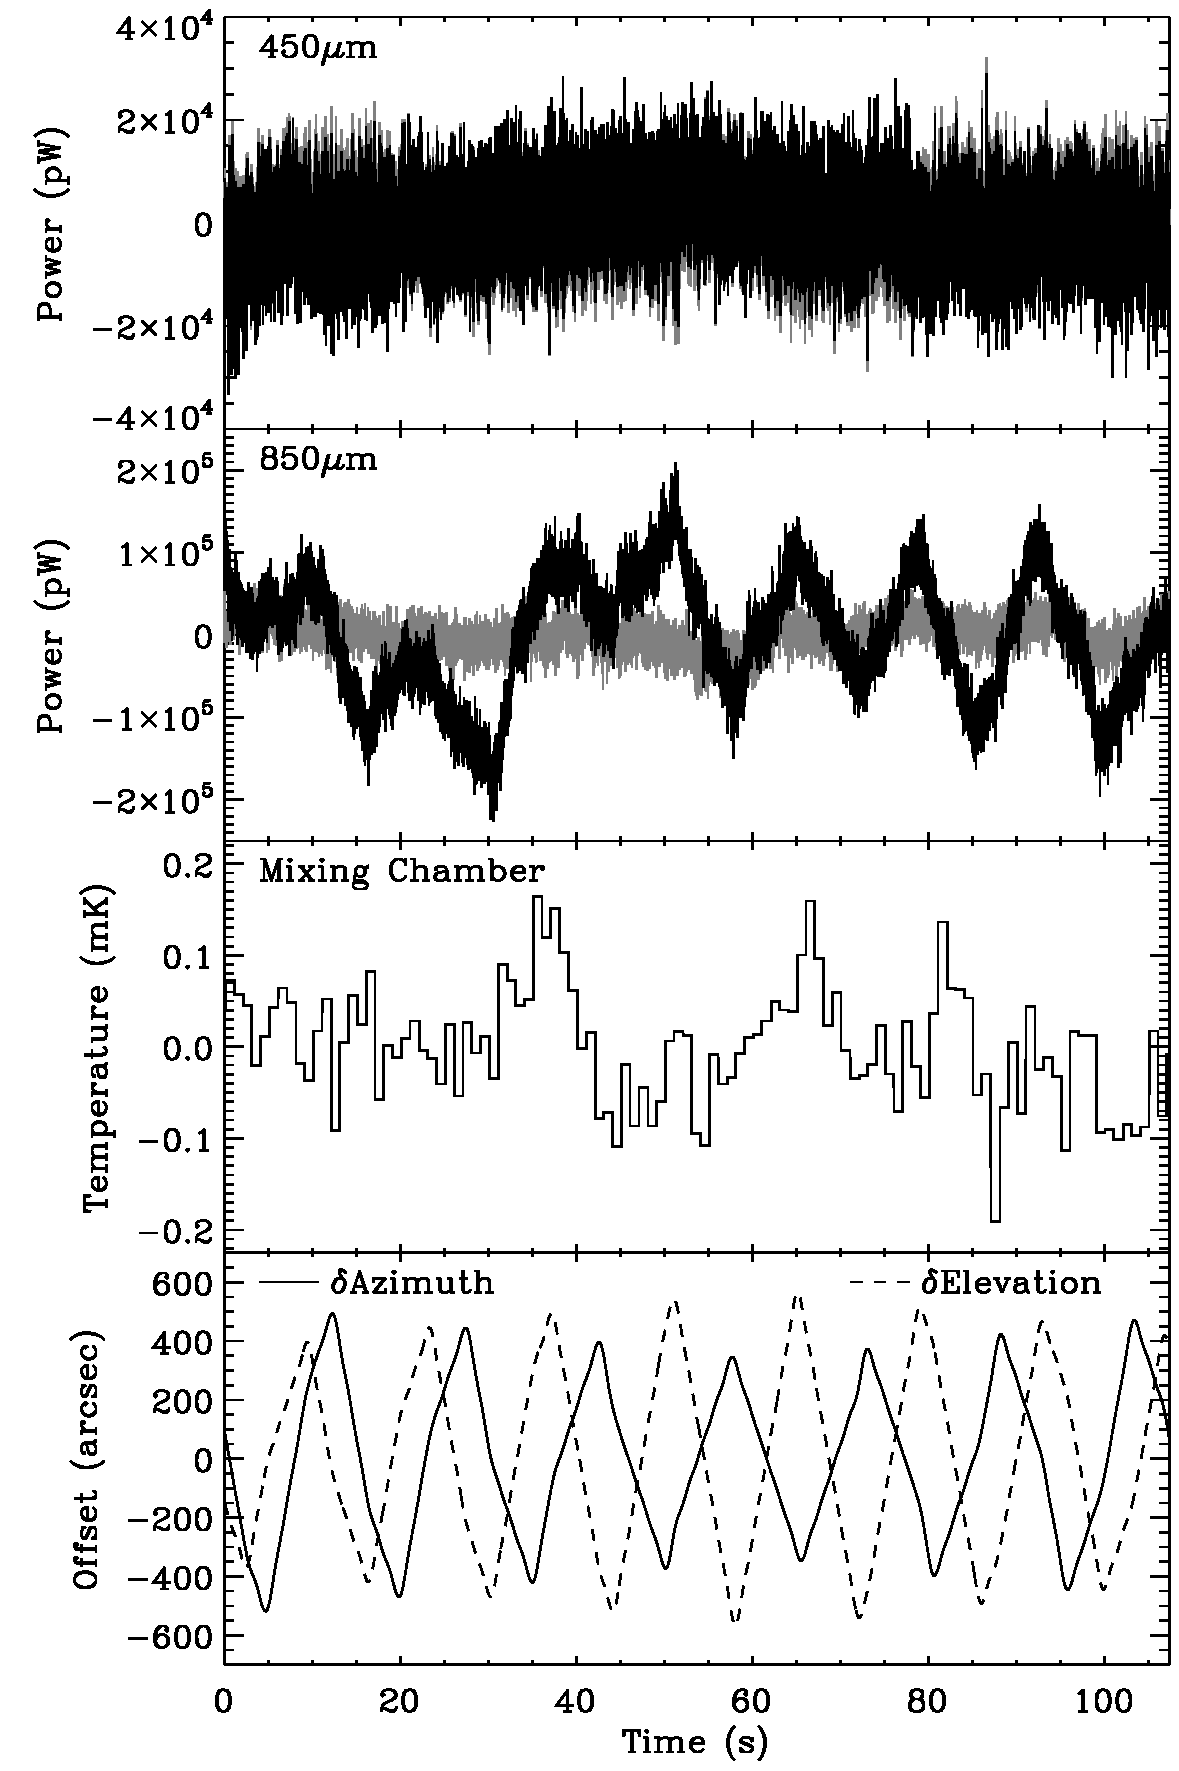
\includegraphics[width=\linewidth]{bolos_point_mix.pdf}
\caption{A comparison between single bolometer time series in each
  band (top two plots), with the mixing chamber temperature and
  azimuth/elevation pointing offsets. There is a strong correlation
  between the bolometers and the roughly $\sim$25\,s oscillation in
  the fridge, but not with the telescope motion. Also note that the
  total power in this primary signal is similar at both 450 and
  850\,\micron, pointing to an internal rather than an external
  source. The grey signals overplotted in the top-two panels show the
  residual time-series after removing the common-mode signal. This
  operation shows: (i) that most of the low-frequency signal is common
  to all of the bolometers; and (ii) the non-correlated, and
  predominantly white noise at 450\,\micron\ is significantly larger
  than at 850\,\micron.}
\label{fig:bolos_mix}
\end{figure}

Both bolometers share significant long-timescale structure
($\gsim10$\,s) that appears to be related to variations in the fridge
base temperature, although the similarity is clearly greater at
850\,\micron. In this particular case, the total power in the
fluctuations at 450\,\micron, from $-0.04$\,pW to $+0.08$, are larger
than the $-0.03$\,pW to $+0.05$\,pW fluctuations at 850\,\micron. Such
behaviour might be expected if there is a comparable varying thermal
load from the fridge at each wavelength, but a larger contribution of
astmospheric variations through the 450\,\micron\ bandpass filters. We
also note that there is no obvious strong correlation between the
low-frequency signal structure at either wavelength at the telescope
motion.

The low-frequency signal component of the bolometer signals is also
highly correlated amongst bolometers in the same subarray. We have
calculate a common-mode signal, $\mathbf{c}(t)$ as the straight
average time series of all the working bolometers. We then fit the
amplitude of $\mathbf{c}(t)$ at each wavelength to the time series
shown in Fig.~\ref{fig:bolos_mix} and remove it, yielding the grey
residual signals. These residuals are quite flat, although still with
noticeable variations. The white noise is also apparent, and larger at
450\,\micron\ as one would expect from the larger loading compared to
850\,\micron.

\subsubsection{Power spectral densities}
\label{sec:psd}

Next, we produce power spectral density (PSD) plots for several
representative bolometers in Fig.~\ref{fig:pspec}. To produce this
figure, we follow the convention that the PSD as a function of
frequency, $\mathbf{P}(f)$, is normalized such that the integral over
frequency gives the same variance as the time-series variance across
the full time series. In other words, given a bolometer signal
$\mathbf{b}(t)$,
%
\begin{equation}
\label{eq:psd}
\langle\mathbf{b}^2(t)\rangle = \int \mathbf{P}(f) df .
\end{equation}
%
However, we only show the PSD up to the Nyquist frequency, so the
conversion from variance measured in the frequency domain to the time
domain requires and additional multiplcation by 2; hence the units are
pW$^2$\,Hz$^{-1}$ rather than pW$^2$\,s.

\begin{figure}
\centering
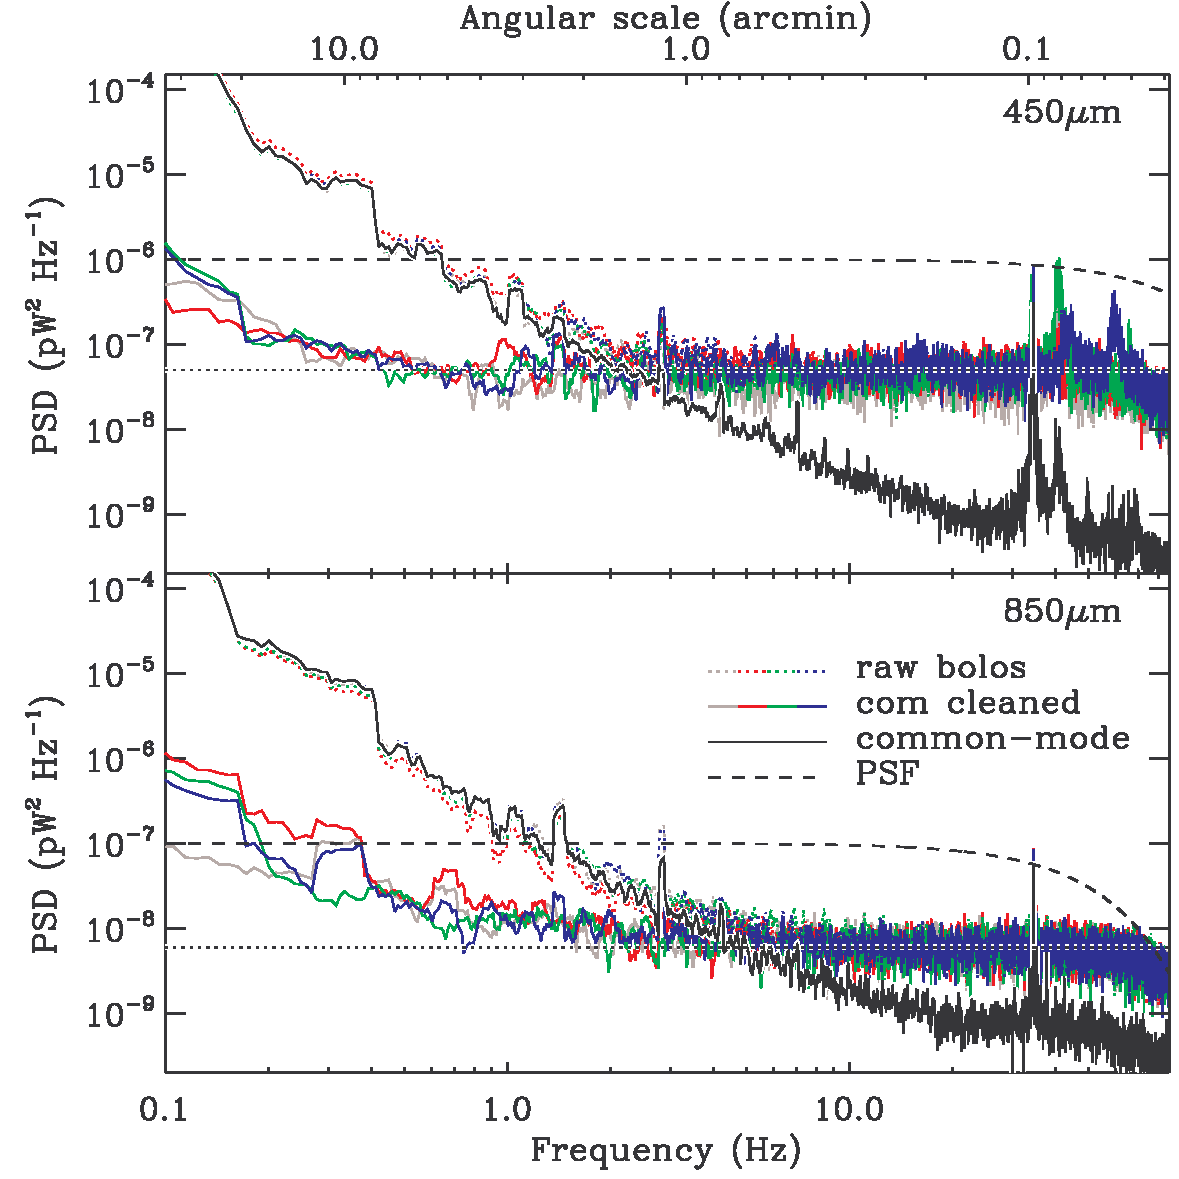
\includegraphics[width=\linewidth]{pspec.pdf}
\caption{Bolometer power spectral densities. Four representative
  bolometers have been selected from each sub-array, and the
  flat-fielded (but otherwise raw) PSDs are shown as coloured dotted
  lines (the blue signals are for the same time series as those shown
  in Fig.~\ref{fig:bolos_mix}). Horizontal dotted lines at $5 \times
  10^{-8}$ and $5 \times 10^{-9}$\,pW\,Hz$^{-1}$ at 450 and
  850\,\micron\ respectively, give the approximate white-noise
  levels. There are broad line features in the PSDs at both
  wavelengths above $\sim$35\,Hz. From $\sim$50\,Hz up to the Nyquist
  frequency, the gradual roll-off of the anti-aliasing filter is also
  evident.  At lower frequencies, the bolometer signals exhibit clear
  $1/f$ knees at approximately 2 and 4\,Hz at 450 and
  850\,\micron. The solid black lines are the PSDs of the common-mode
  signals at each wavelength, and the solid coloured lines show the
  PSDs of the bolometers once the common-mode is removed. These
  residual signals have significantly lower $1/f$ knees, approximately
  0.4 and 2\,Hz at 450 and 850\,\micron. Finally, the dashed black
  lines show the spectral shape produced by a point source, assuming
  that the telescope is slewing at 200\,arcsec\,sec$^{-1}$ (typical
  for S2SRO); for reference, the top horizontal axis shows the
  conversion from frequency to angular scale. We can see that the line
  features may add significant noise on the scale of the PSF. We also
  see that, for this scan velocity, the low-frequency noise begins to
  dominate on scales of approximately 8.3 and 1.7\,arcmin; these scales
  are comparable to the array footprint.}
\label{fig:pspec}
\end{figure}

The dotted coloured lines show the PSDs for raw, though flatfielded
data. At each wavelength, there is a clear $1/f$ knee at a few Hz,
followed by a predominantly white spectrum punctuated by line features
above $\gsim 30$\,Hz, and finally roll-off caused by the anti-aliasing
filter above $\gsim 70$\,Hz. As indicated in the previous section, the
correlation between the low-frequency components of the different
bolometer signals is large. The solid black lines in
Fig.~\ref{fig:pspec} indicate the PSDs of the common-modes
$\mathbf{c}(t)$ at each wavelength, which reproduce most of the
low-frequency structures, as well as the high-frequency line
features. The $\mathbf{c}(t)$ otherwise drop substantially below the
individual bolometer PSDs at high-frequency as expected if the
bolometers are dominated by un-correlated white noise. Finally, we
note that the amplitudes and slopes of the $\mathbf{c}(t)$ are
similar at both 450 and 850\,\micron. However, since the
450\,\micron\ white noise is larger than at 850\,\micron\ (shown
approximately by the horizontal dotted lines), the $1/f$ knee occurs
at a \emph{lower} frequency at 450\,\micron.

Next, the common-mode signals are fit to each bolometer time series
and removed as in Fig.~\ref{fig:bolos_mix}, and the resulting PSDs are
shown as solid coloured lines. In this example, the residual signals
have $1/f$ knees significantly lower than in the raw PSDs.

For reference, the top horizontal axis has been converted to angular
scale assuming a scan velocity of 200\,arcsec\,sec$^{-1}$ which was
typical of the S2SRO observations. The power spectra of the PSFs in
each band (arbitrary normalized to peak values of $10^{-6}$ and
$10^{-7}$\,pW$^2$\,Hz$^{-1}$ at 450 and 850\,\micron\ respectively)
are also showed as dashed lines for this assumed scan velocity showing
that the smallest features resolvable by the telescope may be slightly
affected by the excess noise in the line features. At the lower
frequency end, the $1/f$ noise dominates at scales $\gsim 2$\,arcmin
in the raw data and $\gsim 10$\,arcmin in the common-mode cleaned data
at 450\,\micron, and at scales $\gsim 1$\,arscmin in the raw data and
$\gsim 2$\,arcmin in the common-mode cleaned data at 850\,\micron.

\subsubsection{Principal component analysis}
\label{sec:pca}

A method that has been employed by teams analyzing BOLOCAM and AzTEC
data to identify and remove low-frequency correlated noise is
Principal Component Analysis
\citep[PCA,][]{laurent2005,scott2008}. While we have not (yet)
included ``PCA cleaning'' as a standard feature of SMURF, we have
performed a preliminary analysis in IDL of some SCUBA-2 data to gain
further insight into the nature of the low-frequency noise. The basic
method is as follows: (i) the covariance matrix is built up for all
pairs $(i,j)$ of the $N$ bolometer time series,
$\langle\mathbf{b}_i(t),\mathbf{b}_j\rangle$; and (ii) an eigenvalue
decomposition is used to identify a new set of statistically
uncorrelated eigenvectors, $\mathbf{\xi}_i(t)$ (i.e. whose covariance
matrix is diagonal), such that each of the bolometer time series is a
linear combination of the eigenvectors, or \emph{components}
i.e. $\mathbf{b}_i(t) = \bar{\mathbf{\xi}} \mathbf{\lambda}_i^T$,
where each row of the matrix $\bar{\mathbf{\xi}}$ is an eigenvector,
and $\mathbf{\lambda}_i^T$ is a column vector containing the
corresponding eigenvalues. For convenience, the $\mathbf{\xi}_i$ are
normalized by their \rms, so that the amplitude of each component is
stored in the eigenvalues. In the earlier analyses mentioned, the
low-frequency noise is assumed to be encapsulated in those components
with the largest eigenvalues. Removing the projection of the time
series along those components has been used successfully to reduce
$1/f$ noise while retaining most of the signal in point-like sources.

One unique feature of the SCUBA-2 data is that one can perform a PCA
analysis of both the 450 and 850\,\micron\ data simultaneously. The
first 6 most significant modes of our analysis are shown in
Fig.~\ref{fig:pca}, with the eigenvectors in the top panels, and maps
of the eigenvalues in each subarray in the bottom panels.

\begin{figure*}
\centering
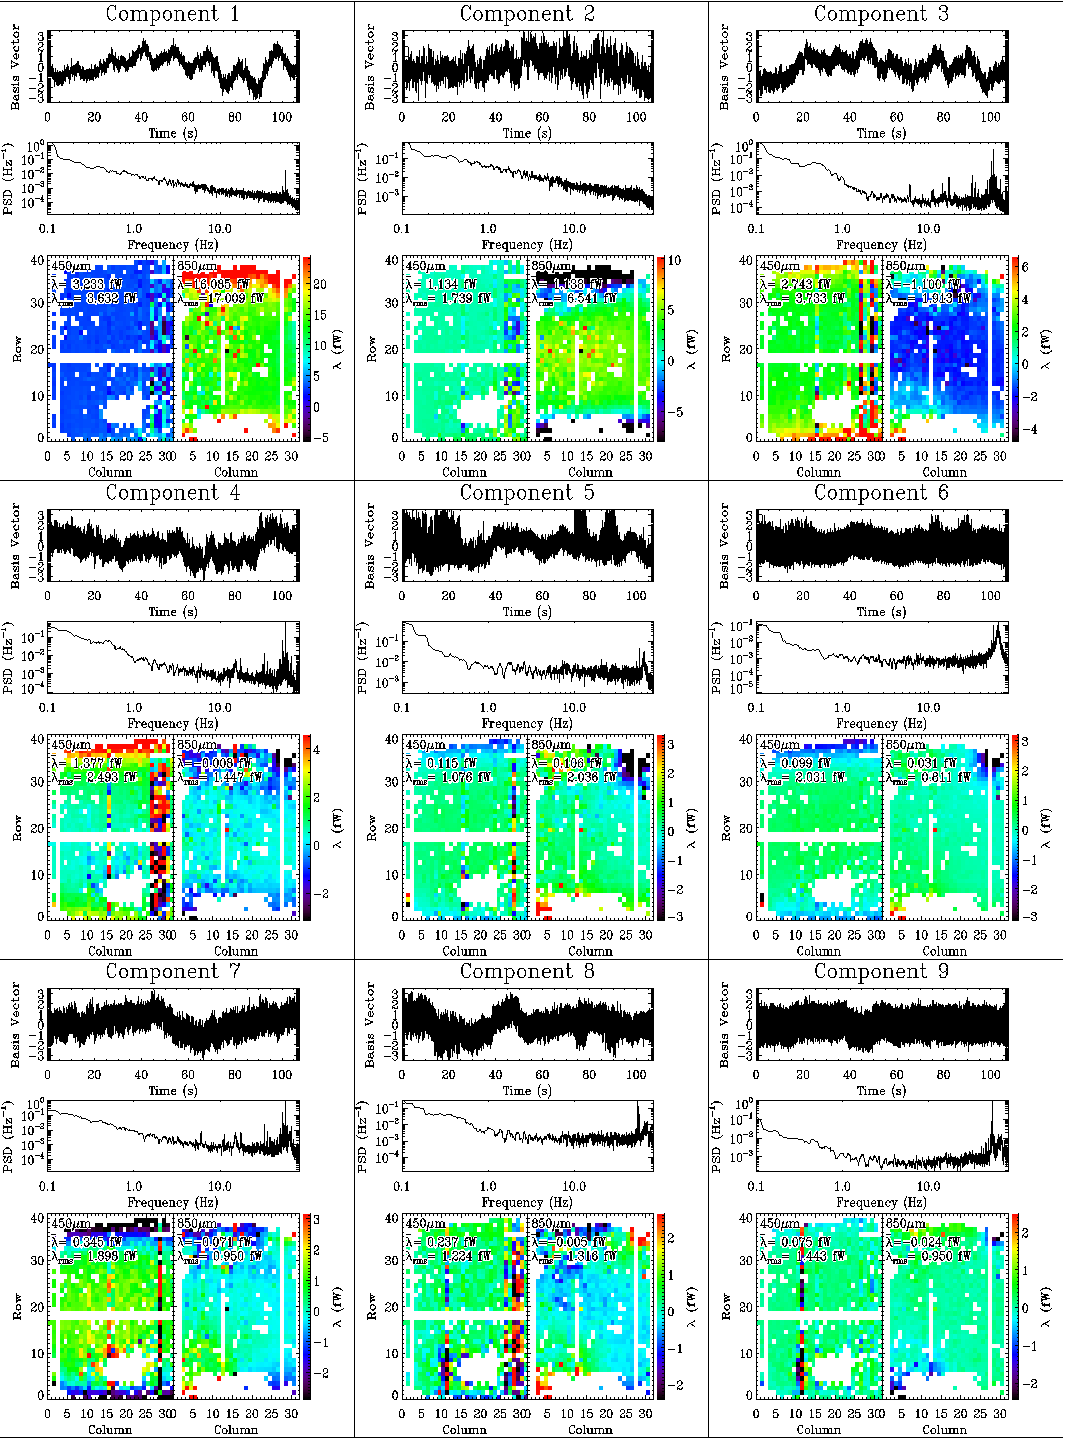
\includegraphics[width=\linewidth]{pca.pdf}
\caption{The first six modes from a principal component analysis,
  ordered by decreasing significance, of the combined 450 and
  850\,\micron\ time-series bolometer data. For each component, the
  top plot shows the time series of the eigenvector, normalized by its
  \rms. The bottom coloured panels show the eigenvalues for the
  bolometers at each wavelength (the amplitude of the eigenvector in
  the time series). For reference, both the mean, $\bar{\lambda}$, and
  \rms, $\lambda_\mathrm{rms}$, eigenvalues for the bolometers in each
  subarray are also shown. The first two components have comparable
  amplitudes, and dominate by at least a factor of 10 any other
  components of the time series. We suspect that they are caused by
  atmospheric variations (expected to be brighter at 450\,\micron),
  and fridge oscillations (expected to be comparable at each
  wavelength). However, the two eigenvectors do not necessarily map
  directly to these physical sources under this interpretation; rather
  they are two \emph{different} linear combinations of the underlying
  physical signals that give rise to statistically uncorrelated
  components. The third component accurately reproduces an apparent
  data-acquisition glitch that appears only at 450\,\micron\ (see
  Section ???). The fourth component is a ...\,Hz line feature only
  observed in column 15 of the 450\,\micron\ subarray. The fifth
  component shows a series of steps and glitches that appear
  predominantly along the bottom-left edge of the 850\,\micron\
  subarray where the bolometers are only tenuously locked. Finally,
  the sixth component is degenerating into a less significant, and
  more randomly scattered signal across the focal plane. Subsequent
  components follow this trend, and would generally be kept in a
  PCA-cleaning procedure.}
\label{fig:pca}
\end{figure*}

The majority of correlated signal at both wavelengths is clearly
broken down into the first two plotted components. The first dominates
at 450\,micron, whereas the second dominates at 850\,micron. For
reference, the eigenvalues of these two modes are in the range
$\sim1$--4\,pW, whereas the remaining modes have eigenvalues
$\lsim0.3$\,pW. As mentioned earlier, one simple model for the
correlated signal is a simple combination of oscillations in base
temperature (which would be similar in each band), with a varying
atmospheric signal (which is expected to be stronger at
450\,\micron). Indeed, the fainter component 2 most closely resembles
the mixing chamber temperature variations (Fig.~\ref{fig:bolos_mix}),
whereas component 1 is stronger at 450\,\micron\ and does not resemble
the fridge signal as closely.

This physical interpretation of the eigenvectors should, however, be
taken with a grain of salt, since the PCA analysis is really a
statistical black box. Suppose most of the low frequency noise really
could be decomposed into two components, the fridge signal
$\mathbf{F}(t)$, and an atmospheric signal $\mathbf{A}(t)$. The two
eigenvectors obtained from the PCA analysis are simply linear
combinations of $\mathbf{F}(t)$ and $\mathbf{A}(t)$ that are
statistically uncorrelated. Depending on the particular realizations
of these two noise sources, this decomposition may, or may not give
rise to eigenvectors that resemble the two underlying physical
sources. Regardless, similar analyses of a few data sets during S2SRO
give comparable results; most of the signal at both 450\,\micron\ and
850\,\micron\ appears to be produced by two dominant underlying
mechanisms.

The subsequent components identified by the PCA analysis in
Fig.~\ref{fig:pca} vary wildly. Component 3, though not obvious from
its eigenvector plot, is almost a pure ramping waveform that only
appears in the s4a data, and produces the broad line featuress
centered over 45\,Hz and 70\,Hz in the 450\,\micron\ PSDs in
Fig.~\ref{fig:pspec}. In other data sets, this third component has
also often instead exhibited a regularly-spaced series of spikes with
heights quantized into several amplitude families (again, only in the
s4a array). In both cases, the shape and phase of this signal is the
same in each bolometer, although the amplitude (and sign) varies, as
evidenced by the large random scatter in the s4a eigenvalue maps. It
is thought that these features are some sort of data acquisition
glitch as the spikes (when they appear) exhibit the expected point
response function of the anti-aliasing filter. Similarly, component 4
also appears to be a data acquisition glitch in the s4a array,
although along a single column, and with a peak at a lower frequency
of 40\,Hz, and a second feature right at the Nyquist frequency.

The last two components in Fig.~\ref{fig:pca} have an entirely
different character. The amplitudes of both components are greatest in
low-responsivity regions of the two subarrays (lower-right at
450\,\micron\ and bottom-left at 850\,\micron). Bolometers in these
regions of the subarray are probably only tenuously locked, and are
more sensitive to changes in the loading, possibly resulting in the
step and spikes that are seen in component 5. Component 6 is clearly
related to component 5, though with the absence of the steps and
spikes, so that together they seem to represent a continuum of shapes
that are linear combinations of the spikes and steps with the slower
drift evident only in component 6.

\subsubsection{Magnetic field pickup}
\label{sec:magpickup}

An additional noise source that appears to be significant in only a
small subset of the S2SRO data is magnetic field pickup. Since the
bolometer signals are ultimately detected through the amplification of
magnetic fields, any additional changing fields within the cryostat
will also be detected.

An example of an observation where pickup appears to be significant is
shown in Fig.~\ref{fig:magpickup}. The time-series for two
450\,\micron\ bolometers in the same column (not flatfielded) show
that there is a strong signal with a similar shape, but opposite
signs. This behaviour is seen across the entire array. The dark squid
signal for the same columns exhibits a similar shape and
amplitude. Since the dark squid has no thermal absorber or TES
attached to it, this observed signal is not likely to be optical or
thermal in nature (although there can be some crosstalk with the
bolometers...). It is also for this reason that the higher-frequency
noise that appears in the bolometer data (thermal) does not appear in
the dark squid, leading to a significantly higher \snr. The sign of
such a signal is expected to be random in the bolometer time-series
(ask detector person for an explanation).

\begin{figure}
\centering
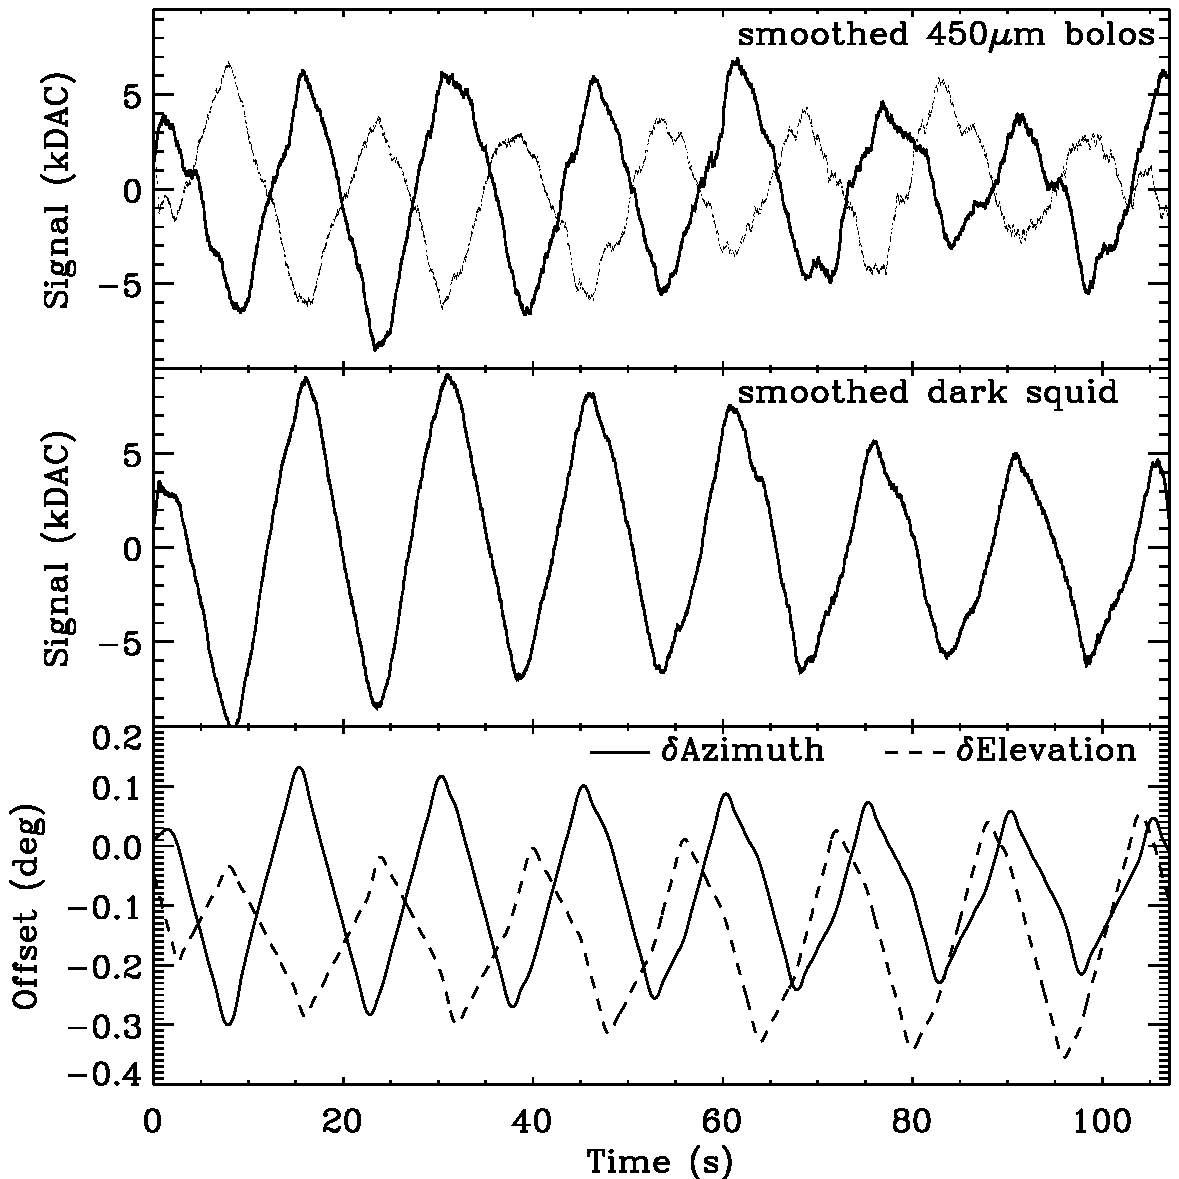
\includegraphics[width=\linewidth]{magpickup.pdf}
\caption{Evidence for significant magnetic field pickup for
  observation 20100228\_00016.  The top panel shows two un-flatfielded
  (but mean-subtracted) bolometer time-series from the same column,
  with a 200 sample boxcar smooth (approximately 1\,s), illustrating
  that they are dominated by a similar signal with opposite signs. The
  second panel shows the dark squid signal for the column, also
  mean-subtracted and with the same boxcar smooth. The bottom panel
  shows the azimuthal and elevation offsets from the map centre. For
  reference, the mean azimuth was 171.9\,deg, and the mean elevation
  68.0\,deg. Only the azimuthal signal appears to be correlated with
  the dark squids and bolometer signals, which suggests a magnetic
  field stationary with respect to the telescope dome as the source,
  since its direction with respect to the cryostat only changes with
  azimuthal motion.}
\label{fig:magpickup}
\end{figure}

The telescope pointing offsets for this approximately 0.5\,deg
diameter scan are also shown in Fig.~\ref{fig:magpickup}. Since the
phase of the azimuth offsets from the map centre in this scan pattern
slowly drifts with respect to the elevation offsets, it is clear that
the bolometer and dark squid signals are detecting a noise source that
is correlated only with the azimuthal motion and \emph{not} the
elevation. This behaviour would be expected if if there were a strong
magnetic field fixed with respect to the telescope dome (i.e., the
earth's magnetic field). Since SCUBA-2 is mounted on a Nasmyth
platform, only azimuthal motion will change the effective direction of
such a field with respect to the cryostat. It is also worth noting
that the absolute azimuth of the telescope was close to 180\,deg
(i.e., nearly due-south). We suspect that this observing
configuration, combined with the large amplitude of the scan, may have
conspired to produce these large signals.

%------------------------------------------------------------------------------
\section{The SMURF Algorithm}
\label{sec:algorithm}
%------------------------------------------------------------------------------

Given predictions for the performance of a fully-functioning SCUBA-2,
and the observed properties of the first-installed subarrays during
commissioning in late 2009 as described in the previous section, SMURF
was designed with two primary goals in mind: (i) reduced maps should
be scientifically useful and of ``near publication quality'' with
minimal user interaction; and (ii) the execution time should not
appreciably exceed the amount of time required to conduct
observations. By attaining these goals it would be possible to conduct
real-time reduction at the telescope to offer feedback to observers,
and it would also be possible to maintain a central repository of
(nearly) publishable data products.

There are two general families of existing map-making strategies that
were considered. The first are \emph{maximum likelihood} methods that
were originally pioneered for the analysis of Cosmic Microwave
Background (CMB) maps. Here, the pixels in the map are considered to
be free parameters in a model-fitting problem, and the data are the
raw time-series. By estimating the full noise covariance matrix for
the data, it is then possible to estimate the maximum-likelihood
map. While direct inversion solutions to this problem are untenable,
some recent efforts to optimize these algorithms have enabled the
reduction of smaller data sets in a reasonable amount of time
\citep[e.g.][]{patanchon2008}. While maximum likelihood maps are,
theoretically, the best maps that can be made from a noise point of
view, the required computing resources and execution time would not
have been feasible for the proposed real-time data reduction and data
archiving model.

\begin{itemize}

\item Describe the bolometer signal model, and with the help of a flow-chart
show the basic procedure that SMURF follows.

\item Discuss SMURF configurability

\item Some sort of proof/demonstration showing why the algorithm works

\item Discuss performance (execution time, memory, disk usage etc.)

\item Where do you get SMURF/starlink, usage of NDF

\item Talk about pipeline?

\end{itemize}

We express the signal observed by the $i$th bolometer as a function of time,
\begin{equation}
\mathbf{b}_i(t) = g_i[\mathbf{e}_i(t) \mathbf{a}_i(t) + \mathbf{n}_i(t)]
\end{equation}
where $\mathbf{a}(t)$ is the time-varying signal produced by scanning
the telescope across astronomical sources, $\mathbf{e}(t)$ is the
time-varying extinction, which is a function of the telescope
elevation and atmospheric conditions, and $\mathbf{n}_i(t)$ represents
sources of noise. The two terms in square brackets, as written, have
units of power delivered to the detectors (pW). The scale factor $g_i$
converts this effective power to the digitized units recorded on disk
(DAC), and in this formulation is assumed to be constant in time.

In practice, $g_i$ is further factored into two components: $g_i = r_i
d$. The responsivity, $r_i$, gives the change in current as a function
of power fluctuations (A\,pW$^{-1}$). There is then a final (and
constant across all bolometers) conversion factor from current to DAC
units, $d$ (DAC/A).

As for the noise, $\mathbf{n}_i(t)$, we break it down into several
components,
%
\begin{equation}
  \mathbf{n}_i(t) = \mathbf{n}^\mathrm{w}_i(t) + \mathbf{n}^\mathrm{f}_i(t) +
  \mathbf{n}^\mathrm{c}(t),
\end{equation}
%
where $\mathbf{n}^\mathrm{w}_i(t)$ is uncorrelated white (thermal)
noise, $\mathbf{n}^\mathrm{f}_i(t)$ is low-frequency noise that is
\emph{not} correlated from bolometer-to-bolometer, and
$\mathbf{n}^\mathrm{c}(t)$ is a (predominantly low-frequency)
correlated or \emph{common-mode} component. The primary goal of
map-making is to model and remove $\mathbf{n}^\mathrm{f}_i$ and
$\mathbf{n}^\mathrm{c}$ from the time-series. By re-gridding the
remaining data we can then hope to approach the theoretical noise
limit in the map. This procedure is summarized in Fig.~\ref{fig:dimm}.

\begin{figure}
\centering
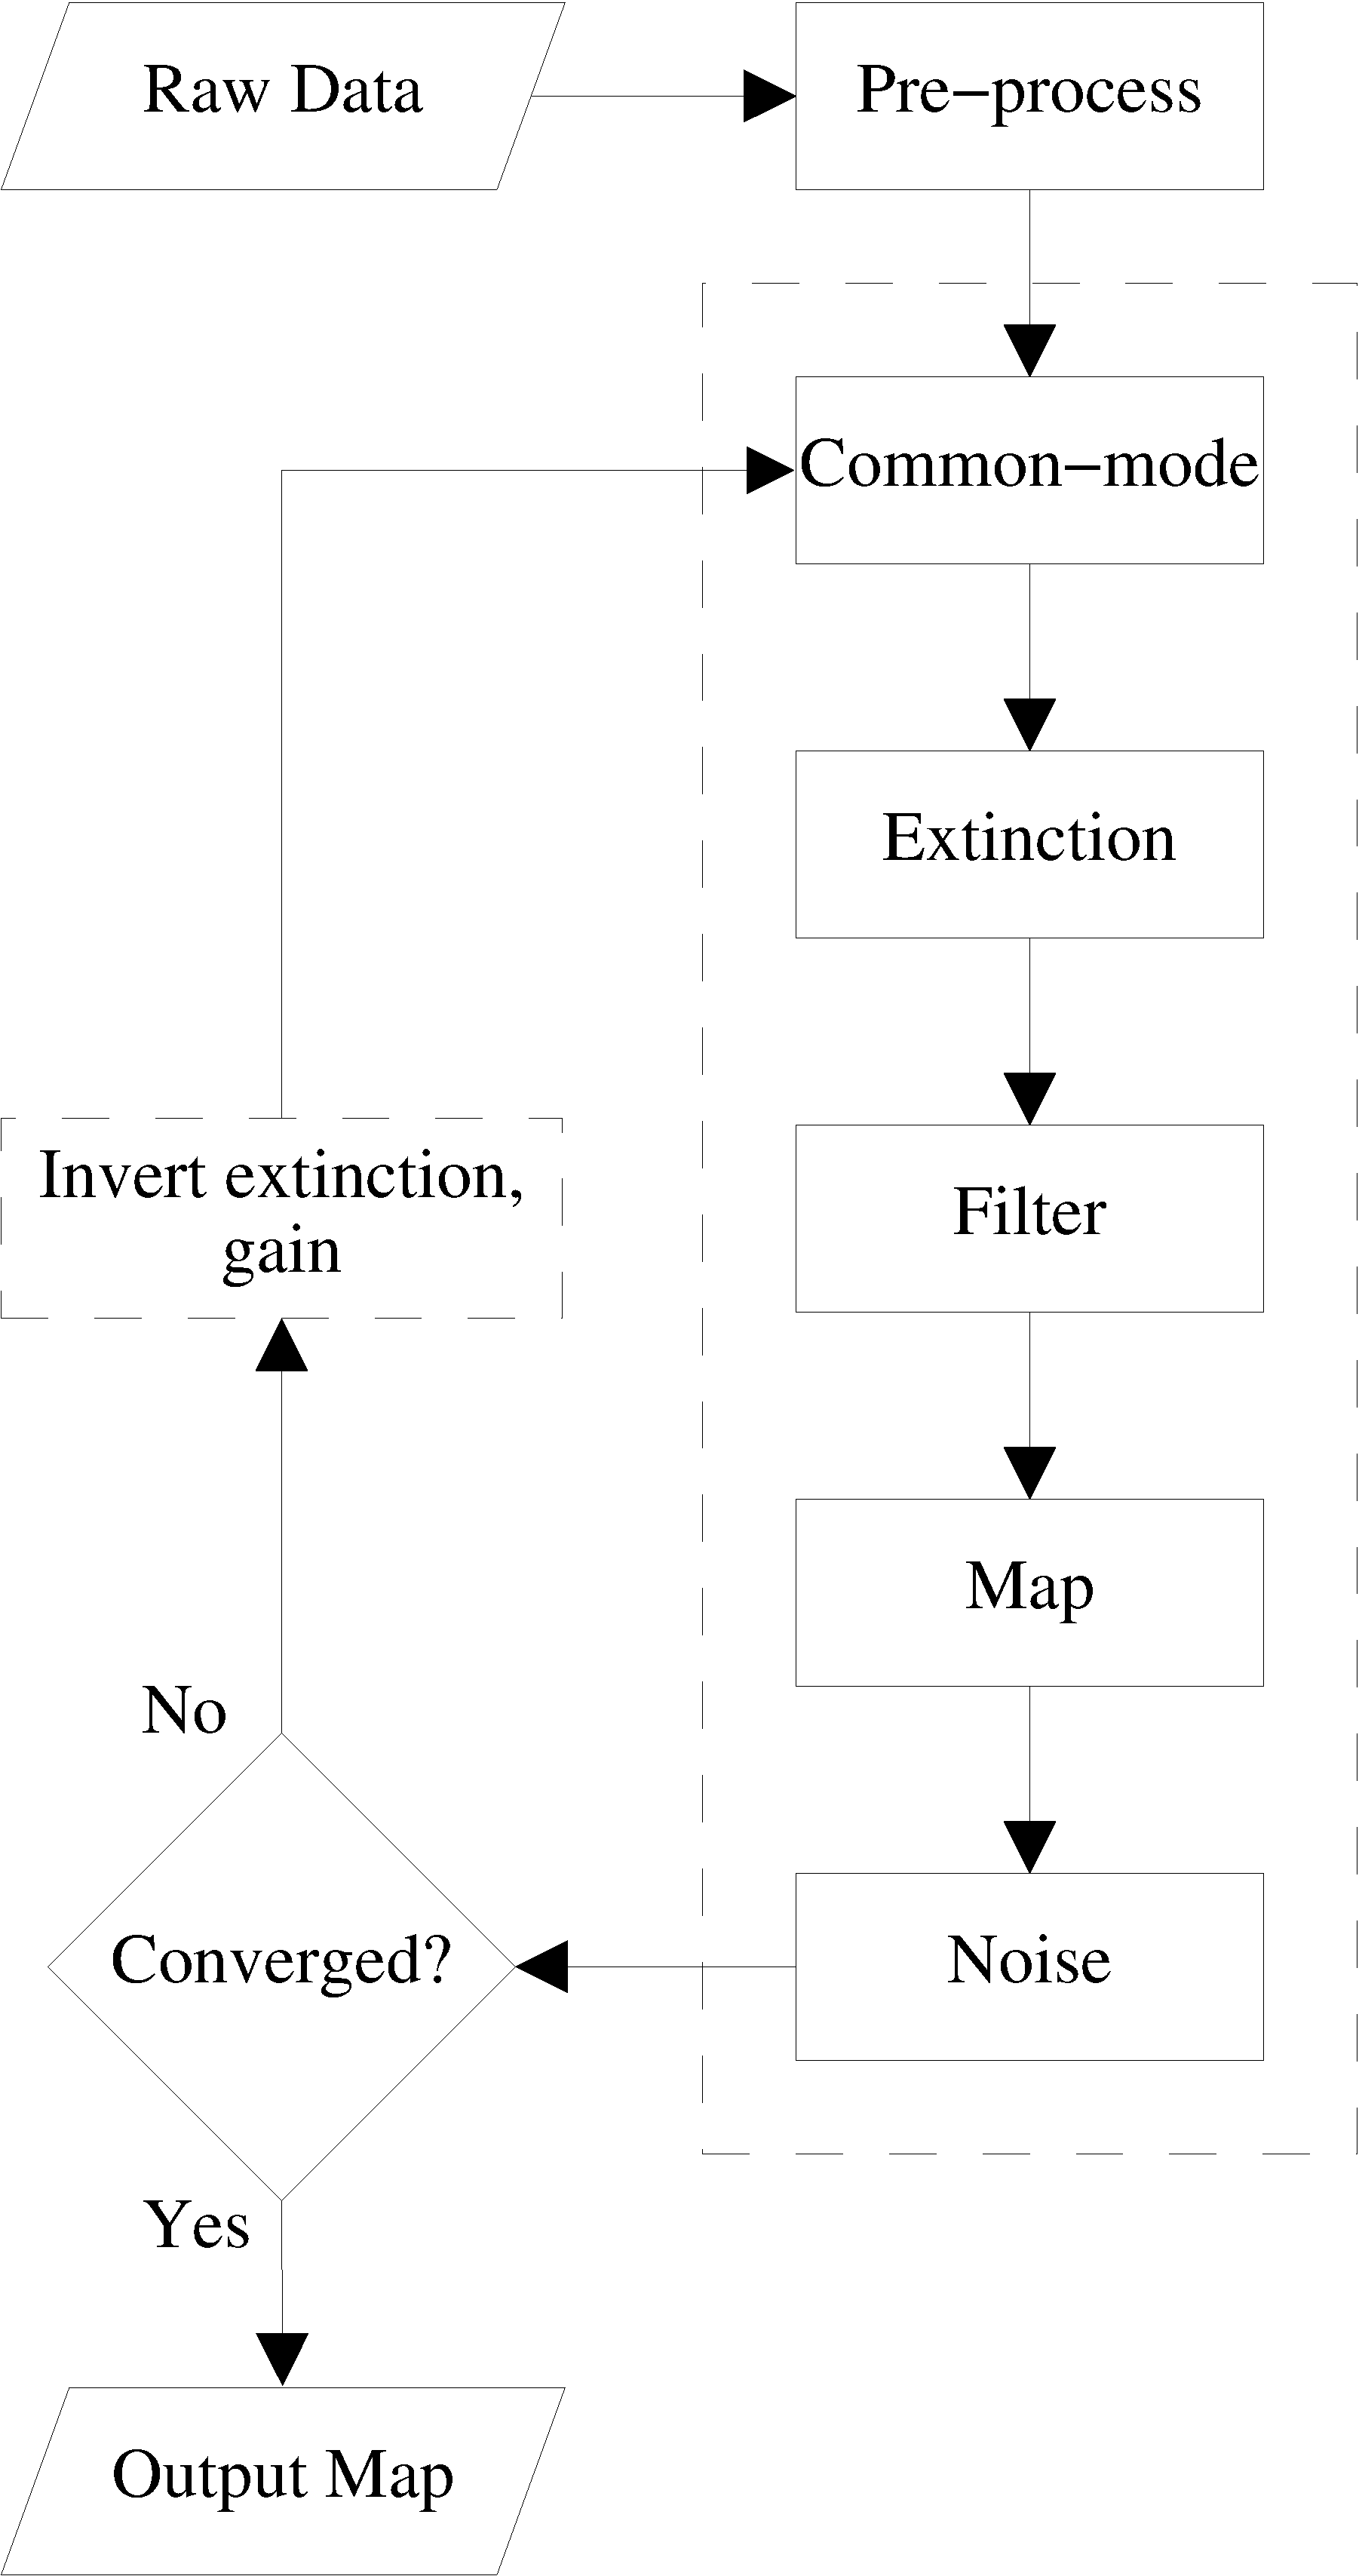
\includegraphics[width=0.75\linewidth]{dimm.pdf}
\caption{Typical map-making algorithm. Raw data (stored in multiple
  files) are read and concatenated into continuous time series. A
  pre-processing stage repairs DC steps, applies a flatfield
  correction, and identifies and removes the noisiest bolometers. The
  iterative portion then begins: estimating and removing the
  common-mode signal; applying the extinction correction; high-pass
  filtering to remove residual independent low-frequency noise;
  estimating the map by re-gridding the data; and finally measuring
  the noise in the residual time series. If the \rms\ has converged,
  the final map is written to disk. Otherwise any multiplicative
  factors that may have been applied to the data are inverted (e.g.,
  extinction correction and relative gains measured during the
  common-mode calculation), and each additive component is added back
  into the time series and re-estimated in turn.}
\label{fig:dimm}
\end{figure}

First, the data files are read from disk, concatenated into contiguous
arrays in memory, and run through a pre-processing stage that performs
several operations including spike and sudden level step removal to
enforce continuity in the time-series. Then, the iterative process
within the dashed box begins. It is generally assumed that the
dominant noise component is the common-mode, which is presumably
dominated by large variations in the fridge temperature and sky noise
(as argued in Section~\ref{sec:pca}). This signal is estimated as the
average signal observed by all of the bolometers at each time step,
and then removed from all of the bolometers. Once this large signal
has been removed, we apply the extinction correction, which is
determined completely from external measurements. Next, residual noise
that differse from bolometer-to-bolometer (primarily low-frequency) is
removed using an FFT-based filter. The resulting ``clean'' time-series
are then re-gridded to produce a map estimate using nearest-neighbour
sampling. Since each map pixel averages many bolometer samples
together, it is fundamentally much less noisy than the bolometer
time-series. We can therefore project the map back into the time
domain, and create relatively noiseless estimates of what each
bolometer would have seen in the absence of noise sources, and remove
that from the time-series. This final step in the iteration gives a
residual signal (with low-frequency and astronomical noise components
removed) that may be used to measured the white noise level in each
detector, and also to estimate an approximate $\chi^2$ for the model
to track convergence. As we will discuss in the next sections, each
signal component estimate is biased slightly from the presence of
signal from other components, so the entire process is
iterated. However, before the next iteration begins, we first undo the
multiplicative factors introduced by the extinction correction, and
also relative gains that may optionally be estimated in the
common-mode estimation phase.

In practice, the map-maker is highly configurable, both in terms of
the order in which model components are fit (and whether they are fit
at all), and the details of \emph{how} they are fit. A summary of the
model components is given in the next section.

%-------------------------------------------------
\subsection{Model components}
\label{sec:components}
%-------------------------------------------------

In addition to specifying when each model component is calculated
(normally an attempt is made to order them by decreasing amplitude in
the time-series), there are a number of parameters that control their
operation. Table~\ref{tab:components} list the model components and
the typical order in which they are calculated. The following sections
describe their implementation in detail.

\begin{table}
  \caption{Summary of the model components that can be fit to
    \scuba\ time-series data with SMURF. Only the first group of
    models are typically fit to the data (\texttt{COM}--\texttt{NOI})
    in the indicated order. The remaining models
    (\texttt{DKS}--\texttt{PLN}) have only been included for
    completeness}
  \vspace{0.2cm}
  \centering
  \begin{tabular}{c|l}
    \hline
    Model & Description \\
    \hline
    \texttt{COM} & remove common-mode signal \\
    \texttt{GAI} & common-mode scaled to each bolometer \\
    \texttt{EXT} & extinction correction \\
    \texttt{FLT} & Fourier transform filter \\
    \texttt{AST} & map estimate of astronomical signal \\
    \texttt{NOI} & noise estimation \\
    \hline
    \texttt{DKS} & dark squid cleaning along columns \\
    \texttt{SMO} & time-domain smoothing filter \\
    \texttt{PLN} & 2-dimensional time-varying plane removal \\
    \hline
    \end{tabular}
  \label{tab:components}
\end{table}

\subsubsection{\texttt{COM,GAI}: common-mode estimation}
\label{sec:comgai}

DSB

We estimate the common-mode, remove it from the time series, use it to
flag bad bits of data, check for time-varying bolometer
responsivities... what doesn't it do?! Also mention the optional
presence of GAI.

\subsubsection{\texttt{EXT}: extinction correction}
\label{sec:ext}

AGG

This is actually only calculated once before the map solution begins
using external opacity monitors (WVM, $\tau_\mathrm{CSO}$,
skydip). Summarize the measurements, order of preference and something
about the calibration for the SCUBA-2 filters.

\subsubsection{\texttt{FLT}: fourier transform filter}
\label{sec:flt}

This model takes the FFT of the bolometer data, and can apply both
high- and low-pass filters, as well as notch filteres, at hard
frequency edges specified by the user. Alternatively, the frequency
edges of the filters may be defined in terms of an \emph{angular
  scale}, but converted into a frequency through knowledge of the mean
telescope slew speed. The time-series may optionally have apodization
applied before the transform to avoid ringing (primarily caused by
wrap-around discontinuities at the ends of the time-series). The
signal that is \emph{removed} from the time-series by this process are
stored in the \texttt{FLT} container array.

\subsubsection{\texttt{AST}: map estimation}
\label{sec:ast}

Map estimation is accomplished using a simple nearest-neighbour
resampling of the data onto a pre-defined map grid. For the $i$th map
pixel $\mathbf{m}(x_i,y_i)$, the brightness is estimated as the
weighted average of the bolometer data samples $\mathbf{b}_j$ that
land within that pixel (from any bolometer or point in time),
%
\begin{equation}
  \mathbf{m}(x_i,y_i) = \frac{\sum_j \mathbf{w}_j \mathbf{b}_j }
                             { \sum_j \mathbf{w}_j } .
\end{equation}
%
For the initial iteration the weights $\mathbf{w}_j$ are set to 1, but
subsequently they are set to $1/\sigma_j^2$, the estimated inverse
variance expected from the bolometer white noise levels as discussed
in Section~\ref{sec:noi}. This weighting scheme is sensible provided
that the bolometer data have no correlated (i.e., low-frequency)
noise.

In addition, a variance map $\mathbf{v}(x_j,y_j)$ is estimated. The
default behaviour is to estimate this weighted error on the mean given
the scatter in the weighted samples. This is accomplished by dividing
the \emph{biased weighted sample variance} by the number of samples
that went into the average (akin to the formula for standard error on
the mean, but accounting for weights),
%
\begin{equation}
\mathbf{v}(x_j,y_j) = \frac{\sum_j \mathbf{w}_j
                            \sum_j \mathbf{w}_j \mathbf{b}_j -
                            \left( \sum_j \mathbf{w}_j \mathbf{b}_j \right)^2 }
                           { N \left( \sum_j \mathbf{w}_j \right)^2 },
\end{equation}
%
where $N_j$ is the total number of bolometer samples that land in the
pixel. We decided not to use the \emph{unbiased} estimator since in
practice it would require accumulating an additional array of values
at every map pixel, and only results in a small difference where there
are less than $\sim10$ samples per pixel (a situation that is almost
never encountered in a SCUBA-2 map except in the edge pixels).

Finally, once the map estimation is complete, the map is projected
into the time domain (the signal that would be produced in each
bolometer by the signal represented by the map) and removed.

In addition to map estimation, the \texttt{AST} model can also be used
to perform map-based despiking of the time-series
(Section~\ref{sec:mapdespike}), and to apply constraints to the map to
improve convergences (Section~???).

\subsubsection{\texttt{NOI}: noise estimation}
\label{sec:noi}

The primary purpose of the noise component, \texttt{NOI} is to measure
the noise in each bolometer residual once all of the other models have
been fit and removed. This noise may then be used to estimate weights
for the data in subsequent iterations.

As in Section~\ref{sec:psd} the FFT of each bolometer time series is
taken, and the PSD calculated. An average white noise level is then
measured from 2 to 10\,Hz, a relatively clean region that lies above
the $1/f$ knee, but below the high-frequency line features for most of
the bolometer data taken during S2SRO (Fig.~\ref{fig:pspec}). Taking
this constant level for $\mathbf{P}(f)$ we then calculate the expected
variance of the time-series (in approximately 200\,Hz samples) using
Eq.~\ref{eq:psd}. If the bolometer noise were produced purely by
uncorrelated thermal sources (i.e. no other long-scale drifts), with
no high-frequency line features, and without the attenuation at even
higher frequencies by the anti-aliasing filter, this is the
theoretical noise limit of the detectors. These measured variances are
stored, and then used in subsequent iterations to weight the data
points when calculating the map estimate (Section~\ref{sec:ast}).

Since noise estimation is usually calculated as the final step, it is
the cleanest data for which some cleaning operations may be
performed. For this reason \texttt{NOI} can optionally use the
time-domain DC step fixer (Section~\ref{sec:steps}) and spike
detection (Section~\ref{sec:timedespike}).

\subsubsection{\texttt{DKS}: dark squid cleaning along columns}
\label{sec:dks}

Columns share significant magnetic field pickup which is measured by
the dark squids. This model has been included although it makes little
improvement, or injects noise since the magnetic field pickup noise is
generally sub-dominant.

\subsubsection{\texttt{SMO}: time-domain smoothing filter}
\label{sec:smo}

TJ

We also have the SMO filter that's useful for very short scans
because edge effects don't matter so much. Two sorts - median which is
more robust, or mean which is more accurate.

\subsubsection{\texttt{PLN}: 2d time-varying sky noise plane removal}
\label{sec:pln}

TJ

We can remove a plane at each timeslice but it doesn't seem to improve
things. Perhaps refer to other papers that claim to have seen coherent
2d structures in the sky noise?

\subsection{Model degeneracies}

Introduce the topic of model degeneracies here, but defer their
solution to the example sections.

%-------------------------------------------------
\subsection{Data cleaning}
%-------------------------------------------------

Since we can do most of this stuff either as a pre-processing step or
iteratively, I thinks this goes in a generic-sounding subsection. This
can go here, or perhaps earlier?

\subsubsection{Down-sampling}

EC

\subsubsection{Whitening filter}

EC

\subsubsection{Time-domain de-spiking}
\label{sec:timedespike}

DSB

\subsubsection{Step correction}
\label{sec:steps}

DSB

\subsubsection{Gap filling / apodization}
\label{sec:gaps}

DSB

Discuss gap filling, ``new'' window function method, also apodization
and start/end polynomial continuity stuff. Should reference CMB
literature -- in particular look at \citet{stompor2002}.

\subsubsection{Flatfields}
\label{sec:flatfields}

TJ

Discuss heater ramps, normalizing off the common-mode signal
amplitude, astronomical sources, and the internal flatfield source.

\subsubsection{Additional bad bolometer rejection}

TJ

Measuring the noise power spectra and throwing away outliers. Data
flagged bad by the DA system.

\subsubsection{Map-based despiking}
\label{sec:mapdespike}

It is possible to use the map estimate (Section~\ref{sec:ast}) to
provide additional despiking of the time-series. Unlike the
time-domain despiker (Section~\ref{sec:timedespike}), this calculation
uses the scatter in the population of samples used to estimate the map
pixel values (from different times and bolometers) to reject
outliers. This method is more robust against false-positive detections
of bright/compact astronomical sources since transient features in the
time-series are unlikely to occur by chance whenever a bolometer
crosses a specific location on the sky, whereas real astronomical
sources are at fixed spatial locations.

The estimated variance, $\mathbf{v_p}(x_i,y_i)$, of the normalized
weighted samples that land in the $i$th map pixel is simply the biased
weighted sample variance (i.e., the variance map value multiplied by
the number of samples)
%
\begin{equation}
  \mathbf{v_p}(x_i,y_i) = N_i \mathbf{v}(x_i,y_i).
\end{equation}

In order to compare the weighted \emph{differences} between the
samples and the map values, [$\mathbf{b}_j - \mathbf{m}(x_i,y_i)$] to
$\mathbf{v_p}$, they must be scaled appropriately. We define a
normalized difference, $\mathbf{d}_j$, in such a way that the variance
of this new variable gives the weighted sample variance of the
underlying data points,
%
\begin{eqnarray}
  \frac{\sum_j \mathbf{d}_j^2}{N} &=&
  \frac{\sum_j \mathbf{w}_j [\mathbf{b}_j - \mathbf{m}(x_i,y_i)]^2}
       {\sum_k \mathbf{w}_k} \\
   \Rightarrow \mathbf{d}_j^2 &=& \frac{N \mathbf{w}_j [\mathbf{b}_j -
       \mathbf{m}(x_i,y_i)]^2}{ \sum_k \mathbf{w}_k} .
\end{eqnarray}
%
The map-based despiker flags those $\mathbf{d}_j$ that are further
than some threshold number of standard deviations,
$\sqrt{\mathbf{v_p}}$, away from zero so that they are not used in
subsequent iterations.


%------------------------------------------------------------------------------
\section{Examples}
\label{sec:examples}
%------------------------------------------------------------------------------

\subsection{Point source}
Reduce a calibrator. Describe the use of a zero mask around the
source. Compare with \citet{wiebe2009} who used the same method to
constrain a maximum-likelihood map with poor cross-linking.

\subsection{Deep blind survey}
Heavy initial filtering, and only iteratively solve for map and
common-mode with edge constraints.


\subsection{Bright extended emission}
The hardest thing to do with SCUBA-2 at the moment. Try to generate a
source/background mask to assist the map solution based on thresholds
in \snr. Compare with BOLOCAM stuff.

%------------------------------------------------------------------------------
\section{Summary and future work}
\label{sec:summary}
%------------------------------------------------------------------------------

\scuba\ is being re-commissioned. Maybe we will have some initial data
on fridge performance? If both it, and sky noise are relatively
well-behaved, might be able to restrict filtering to lower frequencies
and get larger-scale structures.

Larger array footprint also helps.

Talk about potential of Pascale et al. method to get closer to
max-likelihood map solution (handle maps at constant scan angles with
weights in Fourier space separately).

%------------------------------------------------------------------------------
\section{Acknowledgements}
%------------------------------------------------------------------------------


%------------------------------------------------------------------------------
\bibliographystyle{mn2e}
\bibliography{mn-jour,refs}
%------------------------------------------------------------------------------

%------------------------------------------------------------------------------
\appendix
\section[]{This is an appendix}
%------------------------------------------------------------------------------


\end{document}
